\section{Protocolo de evaluación e inferencia estadística}\label{sec:inferencia}

La evaluación experimental se organiza en dos etapas metodológicas explícitamente separadas para preservar la trazabilidad de las predicciones primarias: (1) la evaluación fuera de muestra (OOF) primaria sobre $28$ configuraciones frente a $22$ referencias en energía bruta, y (2) la reconciliación de estimandos inferenciales y métricas adimensionales sobre esas mismas predicciones guardadas, junto con los estudios diagnósticos en $D+1$. En ningún caso se alteran ni regeneran las predicciones OOF primarias.

\subsection{Métricas, validación anidada y transparencia de presupuestos}

Para evaluar el desempeño en una flota con coberturas heterogéneas ($251$ a $1\,032$ días útiles) y capacidades entre $9{,}8$ y $388{,}0$~MW, el protocolo congelado emplea como métrica primaria el \textbf{error absoluto medio macro por planta}:
\begin{equation}
\mathrm{MAE}_{\mathrm{macro}}(m) := \frac{1}{M}\sum_{i=1}^{M}\frac{1}{|\mathcal{T}_i^{\mathrm{eval}}|}\sum_{t \in \mathcal{T}_i^{\mathrm{eval}}} e_{m,i,t},
\label{eq:mae_macro}
\end{equation}
donde $e_{m,i,t} = |y_{i,t+1} - \hat{y}_{i,t+1 \mid t}|$ en $D+1$ ($\text{kWh/día}$), $e_{m,i,t} = \frac{1}{H}\sum_{h=1}^{H}|y_{i,t+h} - \hat{y}_{i,t+h \mid t}|$ en esquema recursivo ($\text{kWh/día}$) y $e_{m,i,t} = |Y_{i,t}^{(H)} - \hat{Y}_{i,t}^{(H)}|$ en esquema directo ($\text{kWh}$ totales, reportando además su equivalente normalizado por $H$ en $\text{kWh/día}$). Conviene precisar tres aspectos de escala y nomenclatura: (i) promediar primero por planta iguala la ponderación respecto a la duración de las series ($|\mathcal{T}_i^{\mathrm{eval}}|$), pero al expresarse en $\text{kWh/día}$ los errores absolutos siguen siendo proporcionales a la capacidad instalada de cada central ($9{,}8$ frente a $388{,}0$~MW); (ii) seis centrales de la cohorte (\texttt{3HF5}, \texttt{3IZ6}, \texttt{EPFV}, \texttt{GYPO}, \texttt{MATA}, \texttt{TPUY}) registran ampliaciones escalonadas de capacidad entre $2024$ y $2026$, por lo que el MAE adimensional en factor de capacidad $\mathrm{MAE}_{\mathrm{CF,macro}}$ divide cada error por $24\,000\,C_{i,t}$ (y por $H$ en directos) usando la capacidad vigente al origen; y (iii) la razón relativa respecto a la generación media observada por planta se etiqueta explícitamente como $\mathrm{nMAE}_{\mathrm{rel,gen}}$ para no confundirla con $\mathrm{MAE}_{\mathrm{CF,macro}}$, mientras que $\mathrm{Skill}_{\mathrm{RMSE}}$ se define exclusivamente frente a \texttt{MM30}.

Para controlar el sesgo de selección \cite{varma2006bias,cawley2010overfit} y transparentar las diferencias de presupuesto de búsqueda entre variantes, distinguimos dos niveles de comparación sobre las $28$ configuraciones experimentales (Figura~\ref{fig:validacion_anidada}):
\begin{itemize}
    \item \textbf{Comparación primaria (\texttt{SM-CFHR-Fixed}, $B=0$):} evalúa la configuración fija ($\delta = 1{,}35$, $\alpha_{\mathrm{lin}} = 0{,}01$, $\alpha_{\mathrm{meteo}} = 0{,}10$) sin optimización de hiperparámetros frente a los $22$ modelos de referencia (los cuales emplearon una rejilla acotada de $4$ configuraciones).
    \item \textbf{Comparación secundaria (\texttt{SM-CFHR-HPO}, $B=25$):} evalúa la variante optimizada mediante $25$ ensayos Optuna TPE dentro de cada pliegue externo sobre $3$ particiones causales internas (embargo de $30$ días en $D+1$, $t_{\mathrm{end}} \le t_{\mathrm{val}}$ en multihorizonte, y exclusión espacial estricta en ET). Reportar por separado $B=0$ y $B=25$ evita atribuir a la arquitectura del modelo ganancias que pudieran provenir de un mayor presupuesto de búsqueda.
\end{itemize}

\begin{figure}[!htbp]
\centering
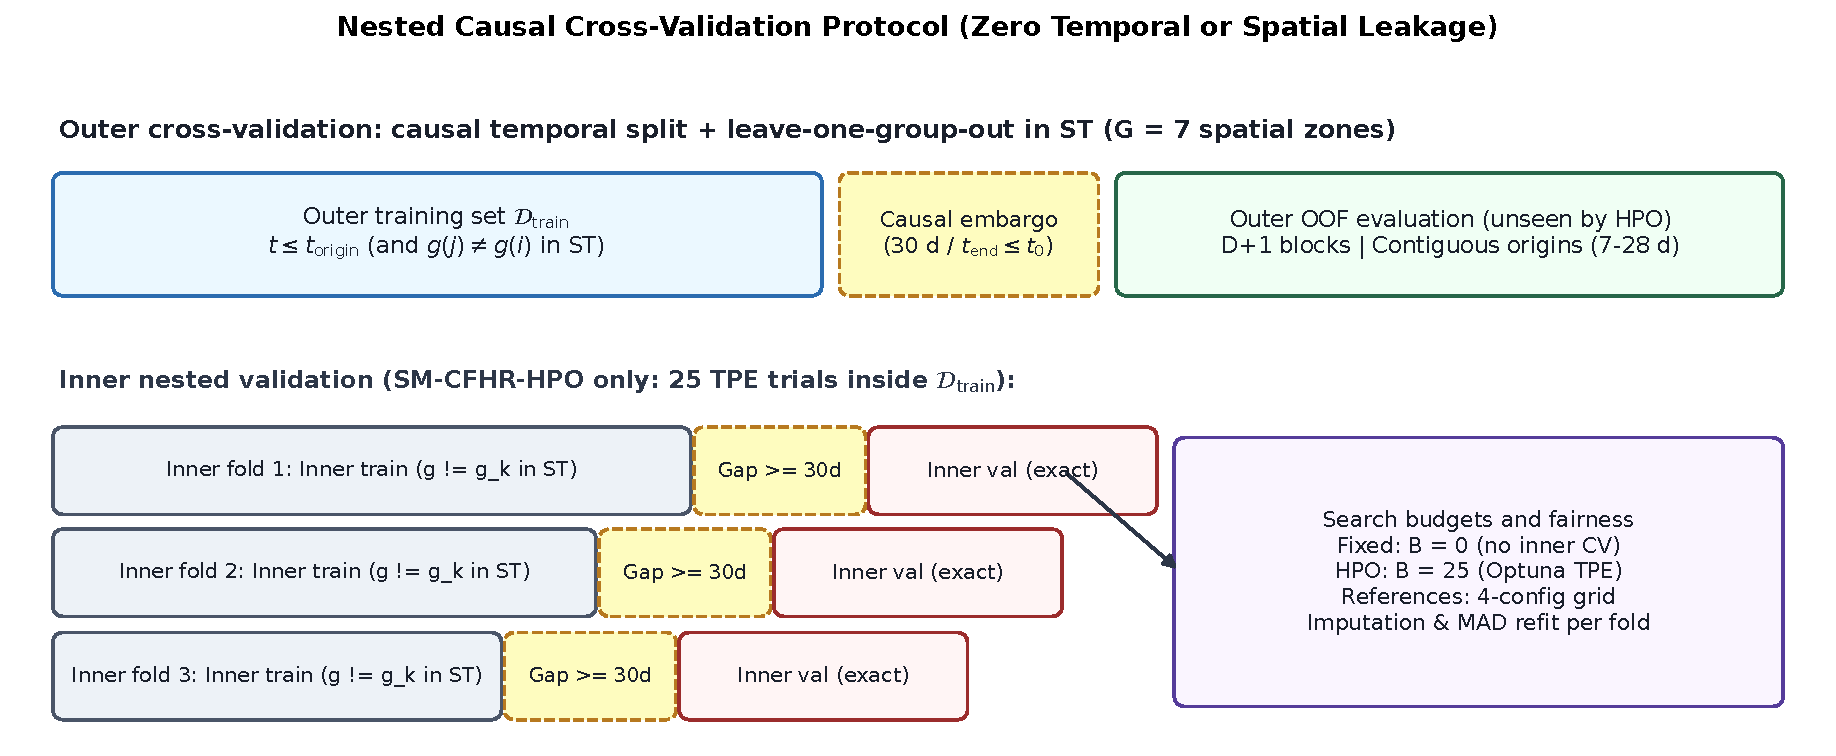
\includegraphics[width=0.98\textwidth]{figures/fig_validacion_anidada.pdf}
\caption{Esquema de validación cruzada causal anidada: separación temporal y espacial externa (\textit{leave-one-group-out} en ET) con brecha de embargo causal de $30$ días y validación interna de $3$ particiones para Optuna TPE.}
\label{fig:validacion_anidada}
\end{figure}

\subsection{Contrastes pareados, multiplicidad y calibración ante autocorrelación}

Para comparar dos procedimientos $m_A$ y $m_B$ sobre series temporales alineadas (agregadas por fecha en $D+1$ y por origen en multihorizonte), definimos el diferencial de pérdida $d_t := L_{m_A, t} - L_{m_B, t}$ para $t = 1,\dots,T$ (valores negativos favorecen a $m_A$). Ante la autocorrelación serial propia de series diarias y de horizontes solapados $H$, la varianza de largo plazo se estima mediante el estimador HAC de Newey--West \cite{newey1987} con núcleo de Bartlett hasta el rezago $L = \max\{1, \lfloor 4(T/100)^{2/9} \rfloor\}$:
\begin{equation}
\hat{\Omega}_{\mathrm{HAC}} := \hat{\gamma}_0 + 2\sum_{k=1}^{L}\left(1 - \frac{k}{L+1}\right)\hat{\gamma}_k, \qquad
\hat{\gamma}_k := \frac{1}{T}\sum_{t=k+1}^{T}(d_t - \bar{d})(d_{t-k} - \bar{d}),
\label{eq:hac}
\end{equation}
y el tamaño muestral efectivo se cuantifica como
\begin{equation}
T_{\mathrm{eff}} := \frac{T}{\max\!\left\{1,\; 1 + 2\sum_{k=1}^{L}\left(1 - \frac{k}{L+1}\right)\frac{\hat{\gamma}_k}{\hat{\gamma}_0}\right\}}.
\end{equation}
Cuando $T_{\mathrm{eff}} < 2H$ (frecuente en horizontes $H \in \{21, 28\}$ días con orígenes no solapados), el protocolo inicial declaraba el escenario con tamaño muestral efectivo insuficiente. La reconciliación inferencial posterior identificó dos desajustes en esa formulación: (a) en los escenarios multihorizonte, los orígenes consecutivos están separados exactamente por $H$ días, por lo que no existe solapamiento entre ventanas ($h_{\mathrm{serie}} = 1$, no $H$); y (b) el promedio simple por origen no coincide con $\mathrm{MAE}_{\mathrm{macro}}$ cuando varía el número de plantas disponibles por origen ($1$ a $17$). Para mantener trazabilidad completa sin alterar las predicciones primarias, la reconciliación añade la serie temporal macro-alineada $z_t^{\mathrm{macro}} = \frac{T}{M}\sum_{i \in \mathcal{P}_t} S_{t,i}/N_i$ (cuya media temporal coincide idénticamente con $\Delta\mathrm{MAE}_{\mathrm{macro}}$), bootstrap estacionario sincronizado entre plantas, política explícita para series de varianza nula ($\Delta=0 \Rightarrow p=1{,}0$; $\Delta \neq 0$ constante $\Rightarrow p=\text{NaN}$, no evaluable por DM asintótico), niveles de fiabilidad muestral según $T_{\mathrm{eff}}$ ($<2h_{\mathrm{serie}}$, $[2h_{\mathrm{serie}},20)$, $[20,30)$, $\ge 30$) y la verificación de SPA/MCS con $B=5\,000$ réplicas (Material Suplementario, Sección~S4).

Sobre los escenarios que superan $T_{\mathrm{eff}} \ge 2H$, se distinguen los procedimientos integrados en la evaluación primaria frente a los análisis complementarios post-hoc:
\begin{enumerate}
    \item \textbf{Diebold--Mariano con corrección HLN y varianza HAC:} estadístico bilateral frente a $t_{T-1}$ bajo $H_0 : \mathbb{E}[d_t] = 0$ \cite{diebold1995,harvey1997,newey1987}. La comparación preespecificada frente a una referencia única corresponde a la línea base causal \texttt{MM30} (y al contraste pareado entre \texttt{SM-CFHR-Fixed} y \texttt{SM-CFHR-HPO}). En cambio, el contraste frente a la «mejor referencia de biblioteca» seleccionada \textit{ex post} sobre la misma muestra de evaluación está sujeto a sesgo de selección posterior que vuelve anticonservadora la calibración nominal; asimismo, las comparaciones frente a representantes individuales de biblioteca (\texttt{Ridge}, \texttt{XGBoost}) tienen carácter exploratorio.
    \item \textbf{Model Confidence Set (MCS):} eliminación secuencial al nivel $\alpha = 0{,}10$ con estadístico $T_{\max}$ sobre los $23$ modelos simultáneos \cite{hansen2011mcs,politis1994stationary} ($B=200$ réplicas en el protocolo inicial y $B=5\,000$ en la reconciliación macro-alineada, con longitud media de bloque $7$). Permanecer en el MCS indica que no existe evidencia al nivel $\alpha = 0{,}10$ para descartar al modelo como inferior respecto al conjunto superviviente, pero no implica automáticamente significancia pareada frente a cada modelo excluido.
    \item \textbf{Prueba global SPA (análisis post-hoc):} contraste de capacidad predictiva superior con recentrado consistente, $B=500$ a $5\,000$ réplicas de bootstrap estacionario y longitud media de bloque $7$ \cite{hansen2005spa}. Cuando una referencia actúa como $H_0$, rechazarla ($p_{\mathrm{SPA}} < 0{,}05$) indica que al menos un competidor la supera; cuando SM-CFHR actúa como $H_0$, no rechazarla no demuestra superioridad ni equivalencia.
    \item \textbf{Giacomini--White (GW) y Clark--West (CW):} GW \cite{giacomini2006tests} se excluye como prueba confirmatoria cuando $\tau=1$ y $|\hat{\rho}_1| > 0{,}15$ tras verificar sobrerrechazo bajo errores $\mathrm{AR}(1)$ ($0{,}2083$ frente a $0{,}05$ nominal en $120$ simulaciones exploratorias); CW \cite{clark2007nested} se reserva estrictamente para modelos anidados.
\end{enumerate}

Para controlar las comparaciones múltiples dentro de cada familia de escenarios, se aplican la corrección secuencial de Holm--Bonferroni \cite{holm1979} (control de FWER) y el ajuste de Benjamini--Hochberg \cite{benjamini1995fdr} (control de FDR) únicamente sobre los escenarios con $T_{\mathrm{eff}} \ge 2H$. La magnitud práctica de las diferencias se cuantifica mediante $\bar{d}$ con intervalo de confianza al $95\%$ por bootstrap estacionario ($1\,000$ réplicas), la $d$ de Cohen pareada y el delta de Cliff no paramétrico \cite{cliff1993dominance}, manteniendo cautela inferencial por tratarse de $G=7$ conglomerados espaciales \cite{cameron2015cluster}.

\subsection{Hipótesis científicas preespecificadas y estudios diagnósticos}

El protocolo contrasta cuatro hipótesis científicas una vez concluidas las evaluaciones fuera de muestra:
\begin{itemize}
    \item \textbf{H1 (Ventaja de normalización en transferencia espacial):} en generalización espaciotemporal (ET), la normalización causal por factor de capacidad reduce el $\mathrm{MAE}_{\mathrm{macro}}$ frente a regresores globales entrenados sin normalización de escala.
    \item \textbf{H2 (Significancia pareada y relevancia práctica bajo dependencia temporal):}
    \begin{enumerate}
        \item \textit{Hipótesis científica principal:} en los escenarios con tamaño muestral efectivo $T_{\mathrm{eff}} \ge 2H$, SM-CFHR reduce el error fuera de muestra respecto a la referencia preespecificada \texttt{MM30} (y, de forma exploratoria, frente a la mejor referencia de biblioteca y rivales representativos).
        \item \textit{Contrastes pareados y corrección múltiple:} se evalúa mediante la prueba DM--HLN--HAC bilateral ajustada por Holm--Bonferroni ($p_{\mathrm{Holm}} < 0{,}05$) y Benjamini--Hochberg dentro de cada familia de escenarios.
        \item \textit{Tamaños del efecto y relevancia práctica:} se reportan como criterios descriptivos complementarios la $d$ de Cohen pareada ($|d_{\mathrm{Cohen}}| \ge 0{,}20$), el delta de Cliff ($|\delta_{\mathrm{Cliff}}| \ge 0{,}147$) y el intervalo al $95\%$ por bootstrap estacionario.
        \item \textit{Procedimientos complementarios de conjunto:} la pertenencia al MCS ($\alpha=0{,}10$, integrado en el flujo OOF) y la prueba SPA (post-hoc) aportan contexto de conjunto, sin combinar todas las pruebas en un único test ni interpretar la supervivencia en MCS o el no rechazo de SPA como demostración de superioridad pareada.
    \end{enumerate}
    \item \textbf{H3 (Contribución de componentes estructurales):} la pérdida de Huber ($\delta=1{,}35$), la regularización anisotrópica ($\alpha_{\mathrm{meteo}} > \alpha_{\mathrm{lin}}$) y las restricciones de monotonía no negativa aportan mejoras verificables o mayor estabilidad ante atípicos respecto a sus versiones ablacionadas.
    \item \textbf{H4 (Compromiso entre configuración fija y HPO):} la optimización bayesiana TPE ($B=25$) mejora o iguala a la configuración fija congelada ($B=0$) en regímenes con señal meteorológica suficiente sin incurrir en sobreajuste por varianza de selección.
\end{itemize}

Para investigar la contribución de cada componente constructivo (H3) y caracterizar el comportamiento del estimador sobre el panel real $D+1$ con corte cronológico estricto ($\max t_{\mathrm{train}} < \min t_{\mathrm{val}}$), se ejecutan los siguientes estudios diagnósticos:
\begin{enumerate}
    \item \textbf{Ablación controlada en $D+1$ ($6$ variantes):} contrasta \texttt{SM-CFHR\_completo} frente a cinco modificaciones sobre el mismo panel y corte: (a) $\delta = 10^6$ para aproximar pérdida cuadrática $L_2$ (\texttt{sin\_huber\_L2}); (b) regularización isotrópica $\alpha_{\mathrm{meteo}} = \alpha_{\mathrm{lin}}$ (\texttt{sin\_l2\_estructurada}); (c) supresión de cotas $w_j \ge 0$ (\texttt{sin\_monotonia}); (d) estandarización externa manteniendo MAD (\texttt{escala\_std\_vs\_mad}); y (e) ajuste directo en energía bruta $\text{kWh/día}$ (\texttt{energia\_bruta\_vs\_cf}).
    \item \textbf{Sensibilidad, semillas y estrés sintético en $D+1$:} barridos unidimensionales sobre $(\delta, \alpha_{\mathrm{lin}}, \alpha_{\mathrm{meteo}})$, estabilidad en $10$ semillas ($2026$--$2035$) y estrés ante contaminación en entrenamiento ($0\%$, $5\%$ y $10\%$ de perturbaciones $\pm 0{,}6$ en factor de capacidad con ruido gaussiano $\sigma=0{,}10$ en predictores).
    \item \textbf{Incertidumbre conforme temporal e interpretabilidad aditiva:} intervalos conformes divididos al $80\%$ y $90\%$ nominales mediante cuantiles de residuos absolutos pasados \cite{vovk2005conformal,lei2018conformal,barber2023nonexchangeable}, e importancia aditiva exacta $\phi_{q,j} = \sigma_y (z_{q,j} - \bar{z}_{\mathrm{train},j})\,\hat{w}_j$.
\end{enumerate}

\subsection{Coste computacional y reproducibilidad}

Sobre las $28$ configuraciones ($14\,625$ unidades por variante, $206\,073$ filas de predicción), \texttt{SM-CFHR-Fixed} ($B=0$) concluyó en $499{,}75$~s ($8{,}33$~min) con $8$ trabajadores, frente a $29\,550{,}3$~s ($8{,}21$~h) de \texttt{SM-CFHR-HPO} ($B=25$) con $12$ trabajadores ($59\times$ mayor tiempo de pared). Las especificaciones completas de hardware, entorno Python, semilla global~$2026$ y tolerancia a fallos figuran en el Material Suplementario (Sección~S4).
